\documentclass[a4paper,12pt,twoside]{memoir}

% Castellano
\usepackage[spanish,es-tabla]{babel}
\selectlanguage{spanish}
\usepackage[utf8]{inputenc}
\usepackage[T1]{fontenc}
\usepackage{lmodern} % Scalable font
\usepackage{microtype}
\usepackage{placeins}
\usepackage[numbers]{natbib}

\RequirePackage{booktabs}
\RequirePackage[table]{xcolor}
\RequirePackage{xtab}
\RequirePackage{multirow}

% Links
\PassOptionsToPackage{hyphens}{url}\usepackage[colorlinks]{hyperref}
\hypersetup{
	allcolors = {red}
}

% Ecuaciones
\usepackage{amsmath}

% Rutas de fichero / paquete
\newcommand{\ruta}[1]{{\sffamily #1}}

% Párrafos
\nonzeroparskip

% Huérfanas y viudas
\widowpenalty100000
\clubpenalty100000

% Imágenes

% Comando para insertar una imagen en un lugar concreto.
% Los parámetros son:
% 1 --> Ruta absoluta/relativa de la figura
% 2 --> Texto a pie de figura
% 3 --> Tamaño en tanto por uno relativo al ancho de página
\usepackage{graphicx}
\newcommand{\imagen}[3]{
	\begin{figure}[!h]
		\centering
		\includegraphics[width=#3\textwidth]{#1}
		\caption{#2}\label{fig:#1}
	\end{figure}
	\FloatBarrier
}

% Comando para insertar una imagen sin posición.
% Los parámetros son:
% 1 --> Ruta absoluta/relativa de la figura
% 2 --> Texto a pie de figura
% 3 --> Tamaño en tanto por uno relativo al ancho de página
\newcommand{\imagenflotante}[3]{
	\begin{figure}
		\centering
		\includegraphics[width=#3\textwidth]{#1}
		\caption{#2}\label{fig:#1}
	\end{figure}
}

% El comando \figura nos permite insertar figuras comodamente, y utilizando
% siempre el mismo formato. Los parametros son:
% 1 --> Porcentaje del ancho de página que ocupará la figura (de 0 a 1)
% 2 --> Fichero de la imagen
% 3 --> Texto a pie de imagen
% 4 --> Etiqueta (label) para referencias
% 5 --> Opciones que queramos pasarle al \includegraphics
% 6 --> Opciones de posicionamiento a pasarle a \begin{figure}
\newcommand{\figuraConPosicion}[6]{%
  \setlength{\anchoFloat}{#1\textwidth}%
  \addtolength{\anchoFloat}{-4\fboxsep}%
  \setlength{\anchoFigura}{\anchoFloat}%
  \begin{figure}[#6]
    \begin{center}%
      \Ovalbox{%
        \begin{minipage}{\anchoFloat}%
          \begin{center}%
            \includegraphics[width=\anchoFigura,#5]{#2}%
            \caption{#3}%
            \label{#4}%
          \end{center}%
        \end{minipage}
      }%
    \end{center}%
  \end{figure}%
}

%
% Comando para incluir imágenes en formato apaisado (sin marco).
\newcommand{\figuraApaisadaSinMarco}[5]{%
  \begin{figure}%
    \begin{center}%
    \includegraphics[angle=90,height=#1\textheight,#5]{#2}%
    \caption{#3}%
    \label{#4}%
    \end{center}%
  \end{figure}%
}
% Para las tablas
\newcommand{\otoprule}{\midrule [\heavyrulewidth]}
%
% Nuevo comando para tablas pequeñas (menos de una página).
\newcommand{\tablaSmall}[5]{%
 \begin{table}
  \begin{center}
   \rowcolors {2}{gray!35}{}
   \begin{tabular}{#2}
    \toprule
    #4
    \otoprule
    #5
    \bottomrule
   \end{tabular}
   \caption{#1}
   \label{tabla:#3}
  \end{center}
 \end{table}
}

%
% Nuevo comando para tablas pequeñas (menos de una página).
\newcommand{\tablaSmallSinColores}[5]{%
 \begin{table}[H]
  \begin{center}
   \begin{tabular}{#2}
    \toprule
    #4
    \otoprule
    #5
    \bottomrule
   \end{tabular}
   \caption{#1}
   \label{tabla:#3}
  \end{center}
 \end{table}
}

\newcommand{\tablaApaisadaSmall}[5]{%
\begin{landscape}
  \begin{table}
   \begin{center}
    \rowcolors {2}{gray!35}{}
    \begin{tabular}{#2}
     \toprule
     #4
     \otoprule
     #5
     \bottomrule
    \end{tabular}
    \caption{#1}
    \label{tabla:#3}
   \end{center}
  \end{table}
\end{landscape}
}

%
% Nuevo comando para tablas grandes con cabecera y filas alternas coloreadas en gris.
\newcommand{\tabla}[6]{%
  \begin{center}
    \tablefirsthead{
      \toprule
      #5
      \otoprule
    }
    \tablehead{
      \multicolumn{#3}{l}{\small\sl continúa desde la página anterior}\\
      \toprule
      #5
      \otoprule
    }
    \tabletail{
      \hline
      \multicolumn{#3}{r}{\small\sl continúa en la página siguiente}\\
    }
    \tablelasttail{
      \hline
    }
    \bottomcaption{#1}
    \rowcolors {2}{gray!35}{}
    \begin{xtabular}{#2}
      #6
      \bottomrule
    \end{xtabular}
    \label{tabla:#4}
  \end{center}
}

%
% Nuevo comando para tablas grandes con cabecera.
\newcommand{\tablaSinColores}[6]{%
  \begin{center}
    \tablefirsthead{
      \toprule
      #5
      \otoprule
    }
    \tablehead{
      \multicolumn{#3}{l}{\small\sl continúa desde la página anterior}\\
      \toprule
      #5
      \otoprule
    }
    \tabletail{
      \hline
      \multicolumn{#3}{r}{\small\sl continúa en la página siguiente}\\
    }
    \tablelasttail{
      \hline
    }
    \bottomcaption{#1}
    \begin{xtabular}{#2}
      #6
      \bottomrule
    \end{xtabular}
    \label{tabla:#4}
  \end{center}
}

%
% Nuevo comando para tablas grandes sin cabecera.
\newcommand{\tablaSinCabecera}[5]{%
  \begin{center}
    \tablefirsthead{
      \toprule
    }
    \tablehead{
      \multicolumn{#3}{l}{\small\sl continúa desde la página anterior}\\
      \hline
    }
    \tabletail{
      \hline
      \multicolumn{#3}{r}{\small\sl continúa en la página siguiente}\\
    }
    \tablelasttail{
      \hline
    }
    \bottomcaption{#1}
  \begin{xtabular}{#2}
    #5
   \bottomrule
  \end{xtabular}
  \label{tabla:#4}
  \end{center}
}



\definecolor{cgoLight}{HTML}{EEEEEE}
\definecolor{cgoExtralight}{HTML}{FFFFFF}

%
% Nuevo comando para tablas grandes sin cabecera.
\newcommand{\tablaSinCabeceraConBandas}[5]{%
  \begin{center}
    \tablefirsthead{
      \toprule
    }
    \tablehead{
      \multicolumn{#3}{l}{\small\sl continúa desde la página anterior}\\
      \hline
    }
    \tabletail{
      \hline
      \multicolumn{#3}{r}{\small\sl continúa en la página siguiente}\\
    }
    \tablelasttail{
      \hline
    }
    \bottomcaption{#1}
    \rowcolors[]{1}{cgoExtralight}{cgoLight}

  \begin{xtabular}{#2}
    #5
   \bottomrule
  \end{xtabular}
  \label{tabla:#4}
  \end{center}
}



\graphicspath{ {./img/} }

% Capítulos
\chapterstyle{bianchi}
\newcommand{\capitulo}[2]{
	\setcounter{chapter}{#1}
	\setcounter{section}{0}
	\setcounter{figure}{0}
	\setcounter{table}{0}
	\chapter*{\thechapter.\enskip #2}
	\addcontentsline{toc}{chapter}{\thechapter.\enskip #2}
	\markboth{#2}{#2}
}

% Apéndices
\renewcommand{\appendixname}{Apéndice}
\renewcommand*\cftappendixname{\appendixname}

\newcommand{\apendice}[1]{
	%\renewcommand{\thechapter}{A}
	\chapter{#1}
}

\renewcommand*\cftappendixname{\appendixname\ }

% Formato de portada
\makeatletter
\usepackage{xcolor}
\newcommand{\tutor}[1]{\def\@tutor{#1}}
\newcommand{\course}[1]{\def\@course{#1}}
\definecolor{cpardoBox}{HTML}{E6E6FF}
\def\maketitle{
  \null
  \thispagestyle{empty}
  % Cabecera ----------------
\noindent
\includegraphics[width=\textwidth]{cabecera}\vspace{1cm}%
  \vfill
  % Título proyecto y escudo informática ----------------
  
  \colorbox{cpardoBox}{%
    \begin{minipage}{.8\textwidth}
      \vspace{.5cm}\Large
      \begin{center}
      \textbf{TFG del Grado en Ingeniería Informática}\vspace{.6cm}\\
      
	  	
\includegraphics[width=0.50\textwidth]{primeBotLogo}
	\\

      \textbf{\LARGE\@title{}}
      \end{center}
      \vspace{.2cm}
    \end{minipage}

  }%
  \hfill\begin{minipage}{.20\textwidth}
    
\includegraphics[width=\textwidth]{escudoInfor}
  \end{minipage}
  \vfill
  % Datos de alumno, curso y tutores ------------------
  \begin{center}%
  {%
    \noindent\LARGE
    Presentado por \@author{}\\ 
    en Universidad de Burgos --- \@date{}\\
    Tutor/es: \@tutor{}\\
  }%
  \end{center}%
  \null
  \cleardoublepage
  }
\makeatother

\newcommand{\nombre}{Mario Alonso Pulgar} %%% cambio de comando

% Datos de portada
\title{PrimeBot}
\author{\nombre}
\tutor{Jesús Enrique Sierra García / César Represa Pérez}
\date{\today}

\begin{document}

\maketitle



\newpage\null\thispagestyle{empty}\newpage


%%%%%%%%%%%%%%%%%%%%%%%%%%%%%%%%%%%%%%%%%%%%%%%%%%%%%%%%%%%%%%%%%%%%%%%%%%%%%%%%%%%%%%%%
\thispagestyle{empty}


\noindent
\includegraphics[width=\textwidth]{cabecera}\vspace{1cm}

\noindent D. Jesús Enrique Sierra García profesor del departamento de Digitalización, área de Ingeniería de Sistemas y Automática y D. César Represa Pérez profesor del departamento de Ingeniería Electromecánica y área de Tecnología Electrónica.

\noindent Expone:

\noindent Que el alumno D. \nombre, con DNI 71301872D, ha realizado el Trabajo final de Grado en Ingeniería Informática titulado PrimeBot. 

\noindent Y que dicho trabajo ha sido realizado por el alumno bajo la dirección del que suscribe, en virtud de lo cual se autoriza su presentación y defensa.

\begin{center} %\large
En Burgos, {\large \today}
\end{center}

\vfill\vfill\vfill

% Author and supervisor
\begin{minipage}{0.45\textwidth}
\begin{flushleft} %\large
Vº. Bº. del Tutor:\\[2cm]
D. Jesús Enrique Sierra García
\end{flushleft}
\end{minipage}
\hfill
\begin{minipage}{0.45\textwidth}
\begin{flushleft} %\large
Vº. Bº. del co-tutor:\\[2cm]
D. César Represa Pérez
\end{flushleft}
\end{minipage}
\hfill

\vfill

% para casos con solo un tutor comentar lo anterior
% y descomentar lo siguiente
%Vº. Bº. del Tutor:\\[2cm]
%D. nombre tutor


\newpage\null\thispagestyle{empty}\newpage




\frontmatter

% Abstract en castellano
\renewcommand*\abstractname{Resumen}
\begin{abstract}

El ASTI Robotics Challenge es una competición de robótica que 
se realiza cada año en la ciudad de Burgos y reúne a competidores 
de diferentes lugares de España.

El Proyecto PrimeBot ha sido concebido con el objetivo de desarrollar una base robótica compacta y altamente versátil. Esta base está diseñada para ser fácilmente adaptable a las diferentes pruebas del ASTI Robotics Challenge, ofreciendo una plataforma robusta y multifuncional. La complejidad y flexibilidad de PrimeBot permiten que se integre sin problemas en cualquier reto, asegurando un rendimiento óptimo en cada prueba de la competición.

PrimeBot utiliza algoritmos de control PID (Proporcional, Integral y Derivativo) para el seguimiento de líneas, lo cual es fundamental en muchas competiciones de robótica. Los parámetros del PID pueden ser ajustados en tiempo real para optimizar el comportamiento del robot en diferentes condiciones de la pista.

Una de las características destacadas de PrimeBot es su capacidad de comunicación en tiempo real a través de Bluetooth. Esto permite a los desarrolladores ajustar y monitorizar diferentes parámetros operativos del robot sin necesidad de detenerlo, facilitando así la calibración y el control durante las pruebas. La comunicación Bluetooth se integra de manera fluida con el sistema de control del robot, permitiendo ajustes dinámicos y recepción de datos en tiempo real.

El selector de programa integrado en PrimeBot permite cambiar entre diferentes modos y funciones del robot sin necesidad de conectar a un ordenador. Esta funcionalidad se implementa a través de un DIP switch, que puede detectar hasta 16 posiciones diferentes. Cada posición puede corresponder a una función específica, desde la calibración de sensores hasta la ejecución de algoritmos complejos de navegación.

\end{abstract}

\begin{center} 

\end{center}

\renewcommand*\abstractname{Descriptores}
\begin{abstract}
Robot autónomo, control bluetooth, página web.\ldots
\end{abstract}

\clearpage

% Abstract en inglés
\renewcommand*\abstractname{Abstract}
\begin{abstract}
The ASTI Robotics Challenge is a robotics competition that takes place every year in the city of Burgos and brings together competitors from different parts of Spain.
The PrimeBot Project has been conceived with the aim of developing a compact and highly versatile robotic base. This base is designed to be easily adaptable to the different tests of the ASTI Robotics Challenge, offering a robust and multifunctional platform. PrimeBot's complexity and flexibility allow it to integrate seamlessly into any challenge, ensuring optimal performance in every event of the competition.
PrimeBot uses PID (Proportional, Integral and Derivative) control algorithms for line tracking, which is critical in many robotics competitions. The PID parameters can be adjusted in real time to optimize the robot's behavior in different track conditions.
One of PrimeBot's outstanding features is its real-time communication capability via Bluetooth. This allows developers to adjust and monitor different operating parameters of the robot without having to stop it, thus facilitating calibration and control during testing. Bluetooth communication integrates seamlessly with the robot's control system, allowing dynamic adjustments and real-time data reception.
PrimeBot's integrated program selector allows switching between different robot modes and functions.

Each position can correspond to a specific function, from sensor calibration to the execution of complex navigation algorithms.

\end{abstract}

\renewcommand*\abstractname{Keywords}
\begin{abstract}
Autonomous robot, bluetooth control, web page.\ldots
\end{abstract}

\clearpage

% Indices

\tableofcontents

\clearpage

\listoffigures

\clearpage

\listoftables
\clearpage

\mainmatter
\include{./tex/1_Introduccion}
\capitulo{2}{Objetivos del proyecto}

A continuación se definen los objetivos que han motivado llevar a cabo este proyecto.

\section{Objetivos generales}\label{objetivos-generales}

\begin{itemize}
\tightlist
\item
 Desarrollar un proyecto de robótica desde cero que permita la evolución y adaptación constante.
\item
 Unificar la forma de ejecutar las pruebas en el ASTI Robotics Challenge.
\item
 Aportar un nuevo enfoque a los proyectos que participan en el Challenge.
\item
 Generar un producto compacto y altamente competitivo en el ASTI Robotics Challenge.
\end{itemize}

\section{Objetivos técnicos}\label{objetivos-tecnicos}

\begin{itemize}
\tightlist
\item
 Desarrollar un algoritmo PID adaptable en tiempo real mediante comunicación Bluetooth.
\item
 Implementar un método que permita ejecutar múltiples pruebas sin necesidad de conectar el robot a un ordenador.
\item
 Utilizar GitHub como plataforma para alojar todo el código y la documentación del proyecto.
\item
 Crear una página web de aterrizaje (Landing Page) para la difusión y conocimiento del proyecto.
\item
 Desarrollar un algoritmo para la solución de pruebas de cuadrícula, con control vía Bluetooth y representación gráfica.
\item
 Crear un algoritmo para la resolución de laberintos, incluyendo la representación gráfica del proceso.
\end{itemize}

\section{Objetivos personales}\label{objetivos-personales}

\begin{itemize}
\tightlist
\item
  Contribuir con soluciones innovadoras a las existentes en el ASTI Robotics Challenge.
\item
  Aplicar y ampliar el conocimiento adquirido durante la carrera.
\item
  Explorar metodologías y herramientas modernas utilizadas en el mercado laboral.
\item
  Adentrarme en el campo de la robótica.
\item
  Profundizar en el desarrollo de proyectos Arduino.
\end{itemize}
\capitulo{3}{Conceptos teóricos}

El desarrollo del proyecto PrimeBot (Figura 3.1) implica abordar diversos aspectos teóricos con un nivel considerable de complejidad. 
A continuación, se detallan los conceptos teóricos clave que sustentan este proyecto, abordando tanto componentes electrónicos como algoritmos fundamentales.
\begin{figure}[h]
	\centering
	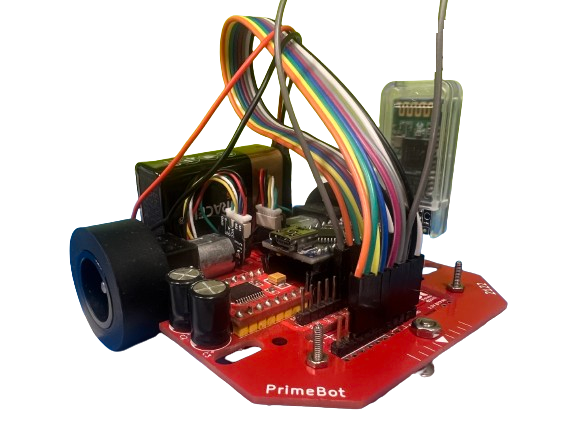
\includegraphics[width=0.5\textwidth]{primebot}
	\caption{PrimeBot}
	\label{fig:3.1}
\end{figure}

PrimeBot se trata de un robot móvil de tracción diferencial ya que dispone de dos ruedas que pueden girar de forma independiente (Figura 3.2).
\begin{figure}[h]
	\centering
	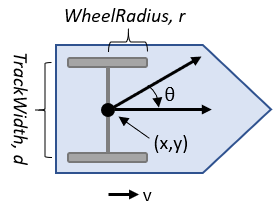
\includegraphics[width=0.25\textwidth]{tracciondiferencial}
	\caption{Modelo de robot de tracción diferencial.}
	\label{fig:3.2}
\end{figure}

\section{Placa de Control}\label{placa-de-control}
PrimeBot está equipado con varios componentes electrónicos esenciales para su funcionamiento y desempeño en las pruebas del ASTI Robotics Challenge. Todo el sistema de PrimeBot está integrado en una Placa de Circuito Impreso (PCB) diseñado específicamente para este proyecto (Figura 3.3) que alberga todos los componentes electrónicos esenciales y facilita su interconexión y gestión.
\begin{figure}[h]
	\centering
	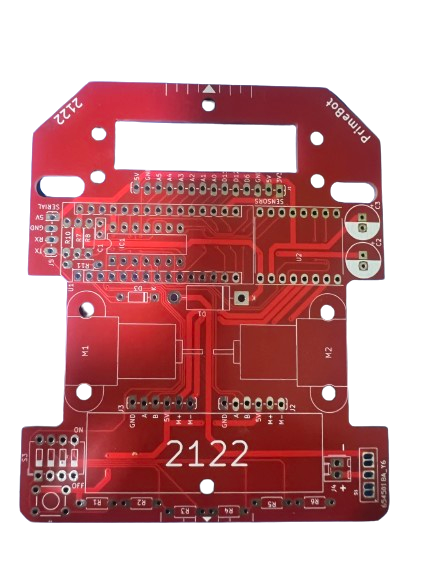
\includegraphics[width=0.20\textwidth]{pcb}
	\caption{PCB}
	\label{fig:3.3}
\end{figure}

\subsection{Arduino Nano Every}\label{arduino-nano}
Arduino Nano Every(Figura 3.4) es un microcontrolador compacto y versátil que actúa como el cerebro de PrimeBot, controlando todos los componentes y ejecutando los programas necesarios para las diferentes pruebas.~\cite{arduinoNanoEvery}
Se ha seleccionado esta placa ya que es el Arduino con el factor de forma más pequeño disponible y tiene un gran número de pines tanto digitales como analógicos para utilizar en todos los sensores que se van a uitilizar en el proyecto.

Además esta placa es una versión mejorada del Arduino Nano convencional, incorporando una mayor cantidad de memoria RAM y memoria Flash que nos permite ejecutar programas más potentes como el que se utiliza en la prueba de la cuadrícula.
\begin{figure}[h]
	\centering
	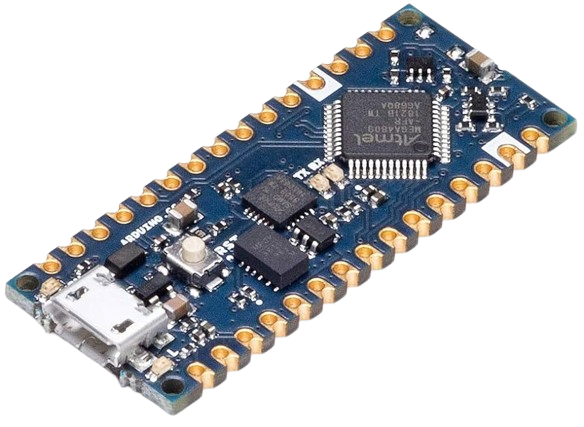
\includegraphics[width=0.25\textwidth]{arduino}
	\caption{Arduino Nano Every}
	\label{fig:3.4}
\end{figure}
\newpage
\subsection{Motores N20}\label{N20}
Motores (Figura 3.5) de corriente continua de alta eficiencia y tamaño compacto, adecuados para aplicaciones que requieren precisión y control.
\begin{figure}[h]
	\centering
	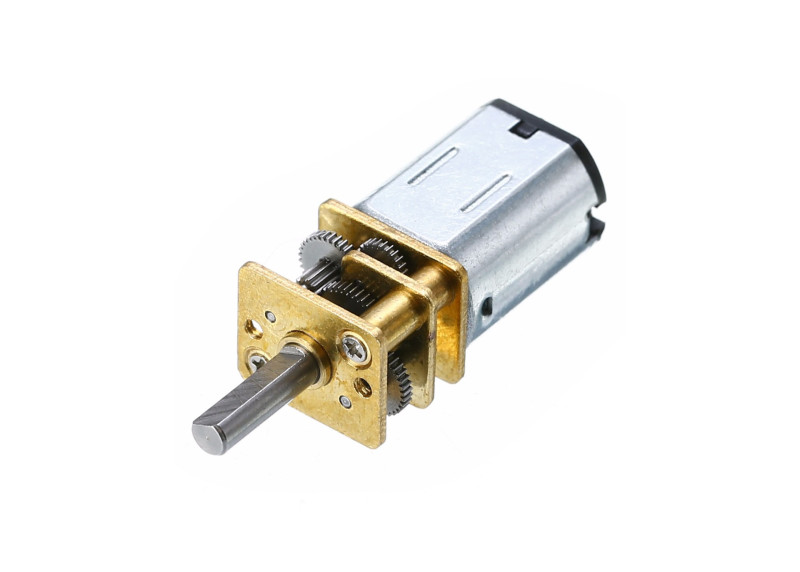
\includegraphics[width=0.25\textwidth]{n20}
	\caption{Motores N20}
	\label{fig:3.5}
\end{figure}


\subsection{Encoders magnéticos}\label{encoders}
Los encoders magnéticos (Figura 3.6) son unos ensores que proporcionan retroalimentación precisa sobre la posición y velocidad de los motores, fundamentales para el control PID.
\begin{figure}[h]
	\centering
	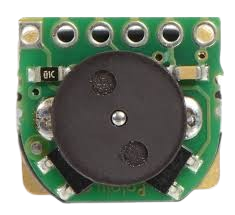
\includegraphics[width=0.2\textwidth]{encoder}
	\caption{Encoders Magnéticos}
	\label{fig:3.6}
\end{figure}

\subsection{Driver de motores TB6612FNG}\label{driver}
Controlador de motores que permite manejar hasta dos motores DC (Figura 3.7), proporcionando una interfaz de control eficiente y protecciones integradas contra sobrecorriente y sobretemperatura.
\begin{figure}[h]
	\centering
	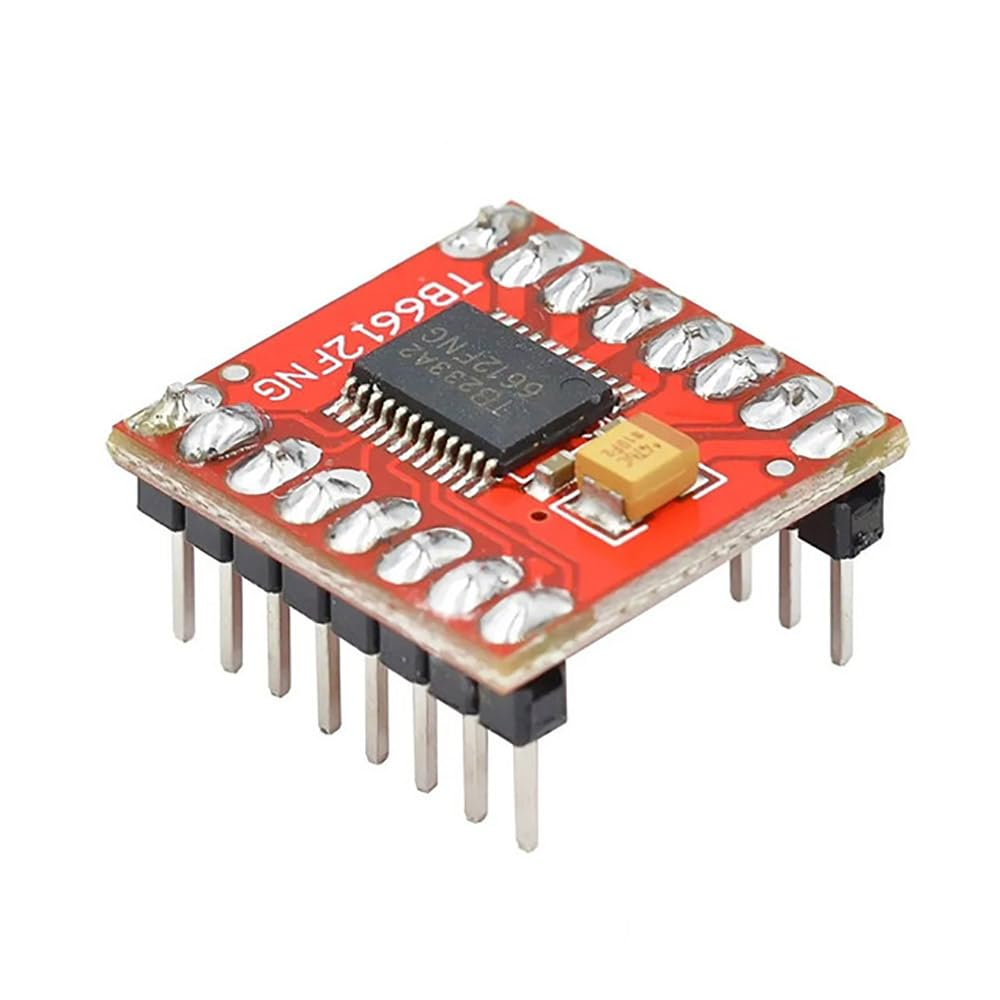
\includegraphics[width=0.2\textwidth]{tb6612fng}
	\caption{Driver de Motores}
	\label{fig:3.7}
\end{figure}

\subsection{Sensores QTR8A}\label{qtr8a}
Sensores de reflectancia utilizados para la detección de líneas en el suelo (Figura 3.8), cruciales para las pruebas de seguimiento de líneas. Estos sensores permiten detectar contrastes entre diferentes superficies, como líneas negras sobre fondos blancos. ~\cite{pololuQTR8A}

\begin{figure}[h]
	\centering
	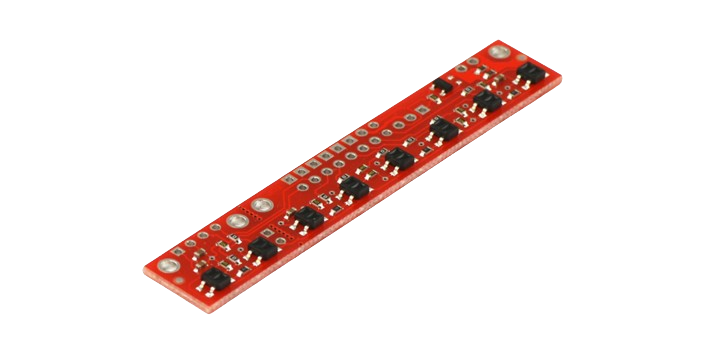
\includegraphics[width=0.5\textwidth]{qtr8a}
	\caption{Sensores de reflectancia QTR-8A}
	\label{fig:3.8}
\end{figure}

\subsection{Pololu OPT3101}\label{opt3101}
Sensores de distancia basados en tiempo de vuelo (ToF) (Figura 3.9) que proporcionan mediciones precisas de distancia, útiles para la navegación y evitación de obstáculos en el entorno del robot. ~\cite{pololuOPT3101}
\begin{figure}[h]
	\centering
	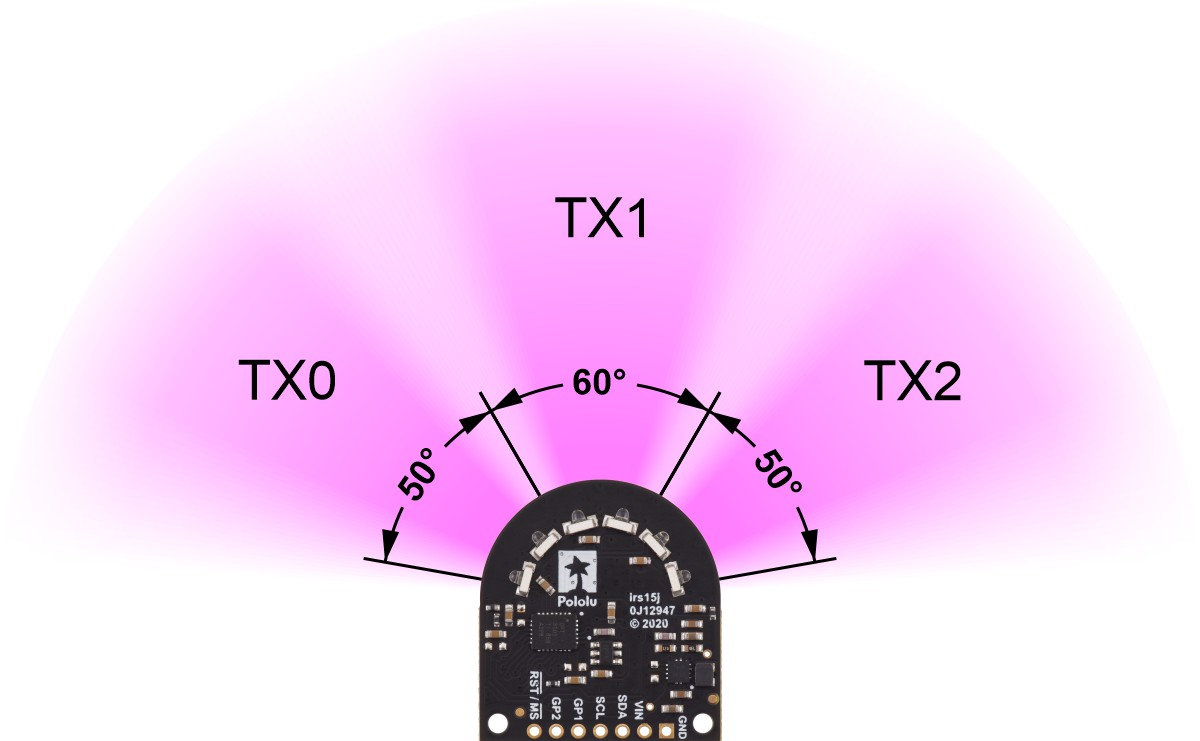
\includegraphics[width=0.5\textwidth]{OPT3101}
	\caption{Sensores de distancia OPT3101}
	\label{fig:3.9}
\end{figure}


\subsection{Selector de posición}\label{selector-de-posicion}
En el PCB de PrimeBot hay un switch mini DIP de 4 posiciones (Figura 3.10) integrado junto a un botón que permite ejecutar el programa correspondiente a la posición seleccionada en el mini DIP.
\begin{figure}[h]
	\centering
	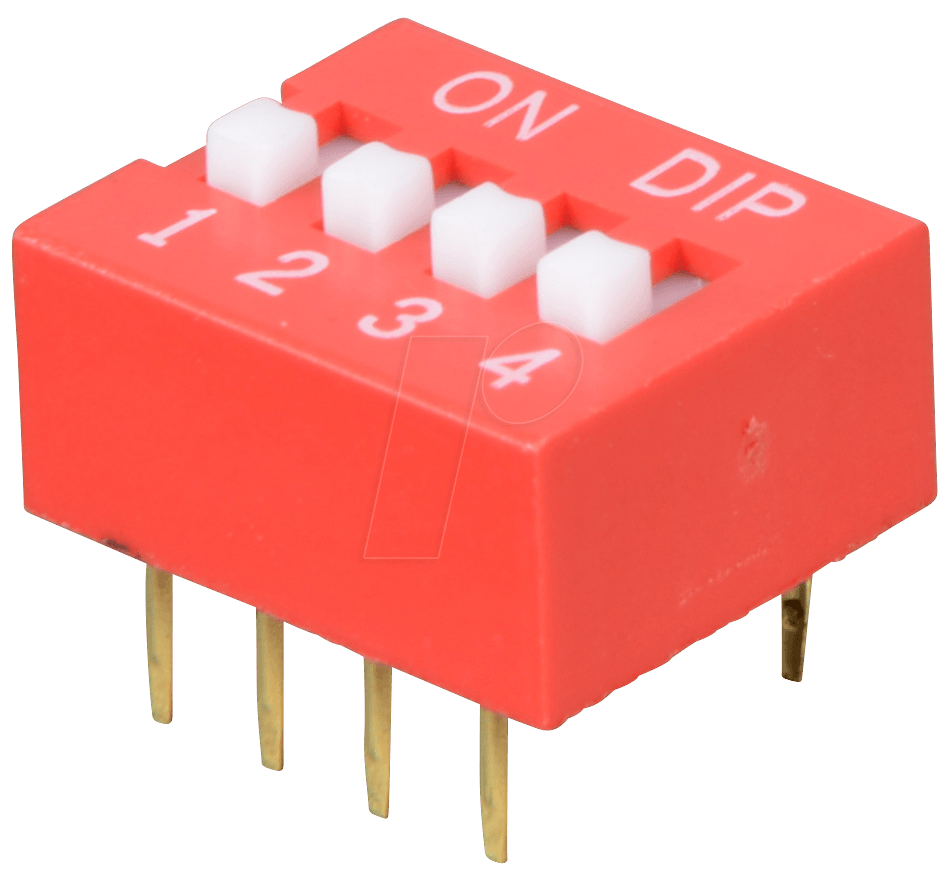
\includegraphics[width=0.25\textwidth]{dip}
	\caption{Switch DIP}
	\label{fig:3.10}
\end{figure}


\subsubsection{Valores del Switch}
El Switch Mini DIP contiene 4 selectores que se pueden mover entre dos posiciones (0 y 1), permitiendo seleccionar desde la posición 0000 hasta la posición 1111, es decir, un total de 15 posiciones diferentes. Esto permite cargar diferentes programas independientes o secciones diferentes de un mismo programa.

El botón situado al lado del Switch proporciona el valor '16' (10000) que el programa 'Main' interpreta como valor de cambio de programa. Esto detiene el programa en ejecución y activa el correspondiente a la nueva posición del switch.

\subsubsection{Uso de Resistencias}
Para que la placa principal de Arduino pueda entender en qué posición está el switch mini DIP, se utilizan una serie de resistencias soldadas en la placa junto a la función de lectura analógica de Arduino. El uso de la lectura analógica de un pin (\emph{AnalogRead()}) dentro de Arduino devuelve un valor de 0 a 1023. Utilizando resistencias de diferentes valores y reflejándolos en el código, Arduino puede interpretar la posición del switch.

El valor de las resistencias es crucial, ya que deben seleccionarse valores bien distanciados para evitar errores en la lectura debido a las tolerancias. Una correcta selección y calibración de estas resistencias asegura una interpretación precisa y fiable de la posición del switch.

En el caso de PrimeBot, para interactuar directamente con el Switch DIP encontramos:
\begin{itemize}
	\item 1 resistencia de 10k ohms
	\item 1 resistencia de 4k7 ohms
	\item 1 resistencia de 2k2 ohms
	\item 1 resistencia de 1k ohms
\end{itemize}

Estos valores están muy distanciados y aproximadamente uno es el doble que el posterior, de esta forma cuando subimos la posición 1 del switch es decir ejecutamos 0001, la resistencia que actúa es la resistencia de 1k ohms y cuando realizamos la lectura correspondiente con \emph{AnalogRead()} obtendremos un valor que será muy diferente al que obtendremos en la posición 0010 que actuará una resistencia de 2k2 ohms y así sucesivamente.
Con el uso de estas resistencias distantes en cuanto a ohms conseguimos realizar lecturas fiables para ejecutar el programa deseado.

\subsection{Integración de Componentes}
El diseño del PCB de PrimeBot está optimizado para integrar todos los componentes necesarios, incluyendo el Arduino Nano, los motores, encoders, sensores y el driver de motores. Esta integración asegura un montaje compacto y ordenado, minimizando las interferencias y facilitando las conexiones.

El PCB también incluye conectores intercambiables para diferentes sensores, lo que permite adaptar fácilmente PrimeBot a las diversas pruebas del ASTI Robotics Challenge. Esta flexibilidad es uno de los puntos fuertes de PrimeBot, permitiendo una rápida configuración y reconfiguración según las necesidades específicas de cada prueba.

\section{Conectividad}\label{conectividad}
PrimeBot incorpora la funcionalidad de conectividad Bluetooth para mejorar la flexibilidad y el control del robot. Esta capacidad permite a los usuarios ajustar los parámetros operativos del robot en tiempo real, sin necesidad de detenerlo ni conectarlo físicamente a un ordenador.

\subsection{Conectividad Bluetooth}
La conectividad Bluetooth en PrimeBot está diseñada para proporcionar instrucciones intuitivas y sencillas para los usuarios. A través de una aplicación compatible o una interfaz serial Bluetooth estándar, los desarrolladores pueden conectarse al robot y modificar configuraciones críticas como las constantes del PID (Proporcional, Integral, Derivativo), la velocidad base y otros parámetros operativos.

\textbf{Uso y Configuración:}
\begin{itemize}
	\item \textbf{Emparejamiento:} Primero, el módulo Bluetooth de PrimeBot debe emparejarse con el dispositivo del usuario (smartphone, tablet, o PC). Este proceso suele implicar buscar dispositivos Bluetooth disponibles, seleccionar PrimeBot y, si es necesario, introducir un código de emparejamiento.
	\item \textbf{Conexión:} Una vez emparejado, se establece una conexión Bluetooth. En este punto, los comandos y datos pueden ser enviados y recibidos.
	\item \textbf{Ajuste de Parámetros:} Mediante comandos simples, el usuario puede ajustar los parámetros operativos. Por ejemplo, enviar 'P+0.1' para aumentar el valor de Kp en 0.1, o 'B+5' para incrementar la velocidad base en 5 unidades.
	\item \textbf{Monitoreo en Tiempo Real:} Los datos del sensor y otros parámetros operativos pueden ser transmitidos de vuelta al dispositivo del usuario, permitiendo el monitoreo en tiempo real y ajustes instantáneos según sea necesario.
\end{itemize}
Esta funcionalidad es especialmente útil durante las competiciones, donde los ajustes rápidos y precisos pueden ser la clave para el éxito. La conectividad Bluetooth facilita también la depuración y el monitoreo del rendimiento del robot, proporcionando una visión inmediata de su estado y comportamiento.


\section{Movimientos y habilidades}\label{movimientos}

\subsection{Algoritmo PID}\label{algoritmo-pid}

Para encontrar un buen equilibrio entre precisión y velocidad el algoritmo utilizado en muchas aplicaciones industriales es el algoritmo PID. ~\cite{ogata2010}

\textbf{El funcionamiento del PID}

El algoritmo PID es un proceso de realimentación en el que un sistema está constantemente recibiendo valores de entrada, en nuestro caso los valores de los sensores.
Con esos valores de entrada el algoritmo PID realiza unos cambios en el sistema que alteran los valores de entrada que va a recibir posteriormente buscando reducir al mínimo el error.

Un algoritmo PID es exitoso cuando se consigue reducir el error al mínimo en todas las lecturas.

Como su nombre indica, el algoritmo PID dispone de tres partes de control principalmente:

\begin{itemize}
	\item \textbf{Parte Proporcional (P):} La parte proporcional es el producto entre la señal del error y la constante proporcional (Kp) proporcionada para que el error se aproxime a cero.
	\item \textbf{Parte Integral (I):} La parte integral tiene como objetivo disminuir el error en estado estacionario y todo lo que no es corregible por la parte proporcional. Se utiliza la constante integral (Ki) como constante a la que multiplicar el error integrado.
	\item \textbf{Parte Derivativa (D):} La parte derivativa tiene en cuenta la tasa de cambio de error proporcionando una acción correctiva basada en la velocidad a la que cambia el error.
\end{itemize}

Además de estas partes, en PrimeBot se incluye también una constante 'Kv' utilizada para optimizar el algoritmo PID en las rectas permitiendo que PrimeBot tenga un mayor rendimiento en zonas donde el error que hay es mínimo aumentando la velocidad.

La fórmula utilizada para el control PID es la siguiente:
\begin{equation*}
	motorSpeedAdjustment = Kp * error + Ki * integral + Kd * derivative
\end{equation*}

\subsection{Seguidor de Líneas}\label{seguidor-lineas}
PrimeBot está diseñado para seguir líneas de manera precisa utilizando el algoritmo PID. 
A continuación, se describen las características, parámetros ajustables y el uso de Bluetooth para el seguidor de líneas.
\subsubsection{Características del Seguidor de Líneas}\label{caracteristicas-seguidor-lineas}

PrimeBot utiliza sensores de reflectancia QTR8A para detectar la línea en el suelo. Estos sensores detectan el contraste entre diferentes superficies, como líneas negras sobre fondos blancos, y envían esta información al microcontrolador. El algoritmo PID procesa estos datos para ajustar la velocidad de los motores y mantener al robot en la trayectoria deseada.

\subsubsection{Parámetros Ajustables por Bluetooth}

Para facilitar el control y ajuste del seguidor de líneas, varios parámetros pueden ser modificados en tiempo real mediante una conexión Bluetooth:
\begin{itemize}
\item \textbf{Constantes PID (Kp, Ki, Kd):} Permiten ajustar la respuesta del algoritmo PID para mejorar el seguimiento de líneas y la estabilidad del robot.
\item \textbf{Constante Kv:} Optimiza el rendimiento en tramos rectos, aumentando la velocidad cuando el error es mínimo.
\item \textbf{Velocidad Base (BaseSpeed):} Ajusta la velocidad base de los motores para controlar la velocidad general del robot.
\end{itemize}

\subsection{Cuadrícula}\label{cuadricula}

PrimeBot está diseñado para navegar y resolver laberintos utilizando una cuadrícula predefinida (Figura 3.11). A continuación, se presenta una explicación teórica de cómo se calculan los movimientos del robot en la cuadrícula, los tipos de movimientos que realiza, la representación gráfica de su trayectoria y los parámetros ajustables a través de Bluetooth.

\begin{figure}[h]
	\centering
	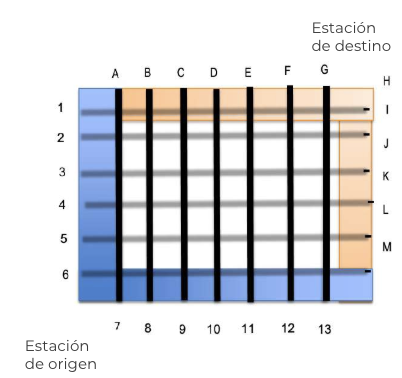
\includegraphics[width=0.25\textwidth]{cuadricula}
	\caption{Ejemplo de cuadrícula}
	\label{fig:3.11}
\end{figure}

\subsubsection{Cálculo de Movimientos}
\begin{itemize}
	\item \textbf{Detección de Cruces:} El robot detecta cruces en la cuadrícula utilizando los sensores QTR, que identifican cuando todos los sensores detectan la línea negra, indicando un punto de intersección.

	\item \textbf{Determinación de la Ruta:} La ruta se determina utilizando las coordenadas de origen y destino. El robot calcula el camino más eficiente evitando puntos bloqueados previamente especificados por el usuario.

	\item \textbf{Actualización de la Posición:} El robot actualiza continuamente su posición en la cuadrícula a medida que se mueve de una celda a otra, utilizando los encoders magnéticos para mantener el seguimiento preciso de sus movimientos.
\end{itemize}

\subsubsection{Movimientos del Robot}
PrimeBot realiza varios tipos de movimientos básicos para navegar por la cuadrícula:
\begin{itemize}
	\item \textbf{Avanzar Una Celda:} El robot se mueve hacia adelante hasta llegar al siguiente cruce.
	\item \textbf{Girar a la Izquierda:} El robot rota 90 grados a la izquierda.
	\item \textbf{Girar a la Derecha:} El robot rota 90 grados a la derecha.
	\item \textbf{Giro en U:} El robot realiza un giro de 180 grados para cambiar de dirección completamente.
\end{itemize}
Estos movimientos son controlados por los motores y ajustados en tiempo real mediante el algoritmo PID para asegurar precisión y estabilidad.

\subsubsection{Representación Gráfica}
PrimeBot genera una representación gráfica de su trayectoria en la cuadrícula, que es visualizada a través de la interfaz serial. La cuadrícula se representa de la siguiente manera:
\begin{itemize}
	\item \textbf{Punto de Salida (S):} Indicado con una 'S' en la cuadrícula.
	\item \textbf{Punto de Destino (D):} Indicado con una 'D' en la cuadrícula.
	\item \textbf{Puntos Bloqueados (X):} Indicado con una 'X' en la cuadrícula.
	\item \textbf{Trayectoria del Robot (*):} Indicado con un '*' en la cuadrícula.
\end{itemize}
La representación gráfica se actualiza en tiempo real para mostrar la posición actual del robot y los puntos recorridos.

\begin{figure}[h]
	\centering
	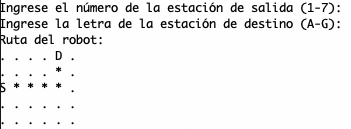
\includegraphics[width=0.50\textwidth]{grafica}
	\caption{Representacion gráfica de la ruta que va a realizar PrimeBot en la Cuadrícula}
	\label{fig:3.12}
\end{figure}

\subsubsection{Parámetros Ajustables por Bluetooth}
Para facilitar el control y ajuste del robot, varios parámetros pueden ser modificados en tiempo real mediante una conexión Bluetooth:
\begin{itemize}
	\item \textbf{Constantes PID (Kp, Ki, Kd):} Permiten ajustar la respuesta del algoritmo PID para mejorar el seguimiento de líneas y la estabilidad del robot.
	\item \textbf{Velocidad Base (BaseSpeed):} Ajusta la velocidad base de los motores para controlar la velocidad general del robot.
	\item \textbf{Coordenadas de Origen y Destino:} Permiten establecer nuevas coordenadas para el punto de salida y el destino, adaptando el recorrido del robot según las necesidades de la prueba.
	\item \textbf{Puntos Bloqueados:} Se pueden definir o actualizar los puntos bloqueados en la cuadrícula, lo que permite al robot recalcular su ruta para evitar estos obstáculos.
	\item El control Bluetooth permite una configuración flexible y rápida, facilitando la adaptación del robot a diferentes escenarios y pruebas del ASTI Robotics Challenge.
\end{itemize}

\subsection{Laberinto}\label{laberinto}

PrimeBot ha sido implementado con la posibilidad de realizar el seguimiento de paredes para poder así resolver laberintos con facilidad.

En resumen, PrimeBot utiliza una combinación de sensores, algoritmos y controladores para calcular y ejecutar movimientos precisos en una cuadrícula, representando su trayectoria gráficamente y permitiendo ajustes en tiempo real a través de Bluetooth para asegurar un rendimiento óptimo en sus tareas de navegación y resolución de laberintos.


\capitulo{4}{Técnicas y herramientas}

\section{Metodologías}\label{metodologias}

\subsection{Scrum}\label{scrum}

Scrum es un marco de trabajo que busca aplicar de manera regular un conjunto de buenas prácticas para el desarrollo de \emph{software}  que se coloca dentro de las metodologías ágiles. En Scrum se realizan entregas parciales y regulares del producto final realizando una estrategia de trabajo iterativa e incremental.

\subsection{Técnica Pomodoro}\label{pomodoro}

La técnica Pomodoro es un método de gestión de tiempo para realizar el trabajo en intervalos incrementando la productividad.
Para aplicar esta técnica se divide la tarea a realizar en intervalos de 45 minutos en mi caso, durante estos 45 minutos se evita cualquier distracción y se descansan 5 minutos al finalizar ese intervalo.
Este periodo de tiempo se conoce como un pomodoro, cada cuatro pomodoros se descansan 30 minutos.

\section{\emph{Hosting} del repositorio}\label{hosting-del-repositorio}

\subsection{GitHub}\label{GitHub}
GitHub es la plataforma web de hospedaje de repositorios más popular en el mundo.
Ofrece todas las funcionalidades de Git y muchas otras integraciones además de ser gratuita.

He utilizado GitHub como plataforma principal donde se va a alojar todo el código del proyecto.

\section{Gestión del proyecto}\label{gestion-del-proyecto}

\subsection{YouTrack}\label{YouTrack}

YouTrack es una herramienta de gestión de proyectos gratuita que permite realizar una implementación SCRUM de forma sencilla.
Gracias a YouTrack podemos trabajar con un tablero canvas y dividir cada sprint en diferentes tareas además de realizar diagramas de Gantt e informes del proyecto.

\section{Entorno de desarrollo integrado
(IDE)}\label{entorno-de-desarrollo-integrado-ide}

\subsection{Arduino IDE}\label{arduino-IDE}

Para el desarrollo del código principal que va incorporado en el microcontrolador de PrimeBot se ha utilizado el IDE Oficial de Arduino.
Este entorno de desarrollo nos aporta todas las herramientas necesarias para llevar a cabo el proyecto, además nos permite trabajar con monitor serial para poder hacer pruebas de conectividad Bluetooth.

\subsection{Visual Studio Code}\label{visual-studio-code}

Visual Studio Code es un editor de código fuente gratuito desarrollado por Microsoft.
Se ha utilizado para realizar el desarrollo de la página web de PrimeBot.

\section{Documentación}\label{documentacion}

\subsection{LaTeX}\label{latex}

LaTeX es un sistema de composición de textos que genera documentos de una gran calidad tipográfica.
Este sistema está muy extendido en el ámbito científico para la generación de artículos y libros. ~\cite{wiki:latex}

TeXShop es un editor de LaTeX y Tex de código abierto para macOS que ha sido utilizado para la redacción de la documentación del proyecto.
\capitulo{5}{Aspectos relevantes del desarrollo del proyecto}

En este apartado se van a recoger los aspectos mas relevantes del proyecto así como los problemas y las decisiones que se tomaron para llevar a cabo con éxito PrimeBot.

\section{Inicio del proyecto}\label{inicio-del-proyecto}

La idea del proyecto apareció en mi cabeza años antes de comenzar tras descubrir con dos amigos el ASTI Robotics Challenge pero sin disponer de tiempo para presentarse a la competencia.
Desde ese año, decidí que en algún momento realizaría un proyecto completo relacionado con ASTI Robotics Challenge.

Arduino ha sido una de las plataformas que más he trabajado en mi tiempo libre y tras recibir el visto bueno de los tutores, llegó el momento de comenzar en el proyecto.

\section{Primeros Pasos}\label{primeros-pasos}

PrimeBot ha resultado ser un reto personal desde el primer día, la idea de realizar algo diferente a lo que se suele ver en la competición no salía de mi cabeza, debido a ello decidí realizar un PCB donde la mayoría de los componentes electrónicos estuvieran soldados.

Gracias al PCB, PrimeBot consigue ser mucho más compacto y ocupar menos espacio que la gran mayoría de soluciones propuestas por el resto de competidores, dotando a PrimeBot de una ventaja en cuanto a agilidad y márgenes de maniobra antes de cometer infracciones en las pruebas.

El primer proceso fue realizar una correcta organización del proyecto utilizando una metodología Ágil como SCRUM para tener unos objetivos marcados y organizados.

\begin{itemize}
\tightlist
\item
  Se siguió una estrategia de desarrollo incremental a través de \emph{sprints} y revisiones.
\item
  La duración media de los \emph{sprints} fue de una semana.
\item
  Al finalizar cada \emph{sprint} se realizaba la publicación de la parte del código correspondiente al sprint.
\item
  En la planificación del \emph{sprint} se generaban unas tareas a resolver en dicho Sprint
\item
  Estas tareas se estimaban y priorizaban en un tablero de la herramienta YouTrack.
\end{itemize}

\section{Programacion de PrimeBot}\label{programacion-primebot}
En el siguiente apartado vamos a tratar los diferentes programas en Arduino que se han creado para el proyecto de PrimeBot.

\subsubsection{5.3.1 Pruebas de componentes}\label{pruebas}
Esta sección consiste en los scripts que se han realizado al comienzo del proyecto, para verificar que el control y el funcionamiento de todos los componentes montados en el PCB funcionaba correctamente.
El proyecto de primeBot dispone de varias pruebas de componentes:

\textbf{Prueba de Selector DIP:} Este script lee la configuración del switch DIP que hay integrado en la placa y determina su valor actual, imprimiendo ese valor a través del monitor serie.
Este script también controla el LED integrado en la placa de Arduino encendiéndolo cuando se detecta el que se ha pulsado el botón de reset.

\textbf{Prueba de motores N20:} Este script utiliza la funcionalidad del switch DIP por lo que es importante verificar que este funciona antes de ejecutar este test.
Aprovechando el Switch DIP se realizan pruebas de movimiento de los motores en todas las direcciones para verificar su correcto funcionamiento.
La acción que harán los motores viene determinada por la posición que tiene el Switch Dip.

\textbf{Prueba de Encoders Magnéticos:} La prueba de los encoders magnéticos consiste en un script que realiza lecturas recurrentes para medir la posición angular en grados.
Los encoders tienen dos señales de entrada que se utilizan para determinar la dirección y la cantidad de rotación.

Gracias al uso de interrupciones, se pueden detectar cambios en las señales del encoder y actualizar un contador que se utiliza para calcular la posición en grados imprimiendo esta posición a través del monitor serie en intervalos regulares.

\textbf{Prueba de Sensores Siguelíneas:}  Los sensores de línea elegidos son los QTR de Pololu, en concreto la placa que contiene 8 sensores analógicos, es decir QTR8A. Este script utiliza la librería de Pololu QTRSensors para gestionar y calibrar los sensores conectados.

Este código utiliza la función \emph{calibrate()} para realizar la calibración de los sensores estableciendo un valor máximo y mínimo leído. Mientras esta función se ejecuta, el LED de la placa de Arduino permanecerá encendido de forma fija y nosotros debemos pasar los sensores sobre la superficie negra y la superficie blanca hasta que termine la calibración.

Una vez temina la calibración, este programa imprime por serial los valores obtenidos en tiempo real de la reflectancia que está obteniendo cada sensor para verificar si está funcionando correctamente.

\textbf{Prueba de Sensores de Distancia:} Los sensores de distancia empleados en la prueba de laberinto pertenecen a pololu siendo los OPT3101.
Este script emplea la libreria creada para estos sensores OPT3101, inicializa el sensor y realiza mediciones de distancia en tiempo real imprimiendo la distancia leida en milímetros a través del monitor serial.

\textbf{Prueba de Bluetooth:}  Este programa inicializa una conexión Bluetooth básica entre arduino y el dispositivo externo. Para comprobar que la conexión Bluetooth se ha establecido correctamente, el usuario puede manejar el parpadeo del LED conectado al pin 13 de la placa Arduino (en este caso es el LED integrado en la placa de Arduino) mediante comandos enviados por el puerto serie.
El usuario enviará un número entre el 1 y el 9 y serán las veces que el LED parpadeará.

\subsubsection{5.3.2 Prueba de "siguelíneas"}\label{siguelíneas}

La prueba de siguelíneas consiste en recorrer un circuito cerrado de una línea negra sobre fondo blanco sin salirte del trazado (Figura 5.1).

\begin{figure}[h]
	\centering
	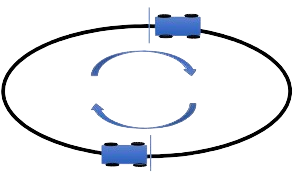
\includegraphics[width=0.50\textwidth]{siguelineas}
	\caption{Circuito para siguelíneas}
	\label{fig:5.1}
\end{figure}

La estrategia más óptima para que PrimeBot pueda realizar esta prueba de forma eficiente es implementando un algoritmo PID (Proporcional, Integral y Derivativo).

\textbf{Algoritmo PID}
 
 El algoritmo PID es un tipo de controlador muy utilizado en sistemas de control. Su objetivo es minimizar la diferencia (el error) entre un valor deseado y el valor real obtenido.
 En nuestro contexto, el valor deseado es que la línea negra esté siempre situada en el centro de los sensores de línea pues en esa posición el error será 0.
 
 Este algoritmo está formado por tres partes:
 \begin{itemize}
\tightlist
\item
  \textbf{Proporcional:} Produce una salida proporcional al error actual, si el error es grande, la salida también lo será.
\item
  \textbf{Integral:} considera la suma acumulada de errores pasados y ayuda a eliminar el error residual que puede persistir si solo se usa la parte proporcional.
\item
  \textbf{Derivativo:} se basa en la tasa de cambio del error, proporciona una predicción de la tendencia del error suavizando la salida.
\end{itemize}

El control PID comienza en PrimeBot con la lectura que se obtiene de los sensores de línea con los que podemos calcular el error de la posición actual.
Cuando ya tenemos el error de posición, podemos calcular la derivada del error (cambio del error con respecto a la lectura anterior)
En la parte integral realizamos la suma acumulativa del error.

Finalmente con las constantes del algoritmo PID y el resto de parámetros calculados realizamos el ajuste en la velocidad de los motores para poder corregir la posición.

Además de este controlador para el seguimiento de la línea, PrimeBot ofrece dentro del código la función \emph{controlador()} que se ha implementado para poder modificar los parámetros del control PID vía bluetooth a través del puerto serial.

Los parámetros configurables son los siguientes:

\begin{itemize}
\tightlist
\item
  \textbf{P:} Aumentará la variable Kp en 0.1
  \item
  \textbf{p:} Reducirá la variable Kp en 0.1
  \item
  \textbf{I:} Aumentará la variable Ki en 0.01
   \item
  \textbf{i:} Reducirá la variable Ki en 0.01
   \item
  \textbf{D:} Aumentará la variable Kd en 0.1
   \item
  \textbf{d:} Reducirá la variable Kd en 0.1
   \item
  \textbf{V:} Aumentará la variable Kv en 0.01
   \item
  \textbf{v:} Reducirá la variable Ki en 0.01
   \item
  \textbf{B:} Aumentará la variable Velocidad base en 1
   \item
  \textbf{b:} Reducirá la variable Velocidad base en 1
\end{itemize}

\subsubsection{5.3.3 Prueba de resolución de cuadrícula}\label{cuadrícula}

La prueba de la cuadrícula consiste en el recorrido desde un punto de origen o estación de origen a un punto de destino o estación de destino.

\begin{figure}[h]
	\centering
	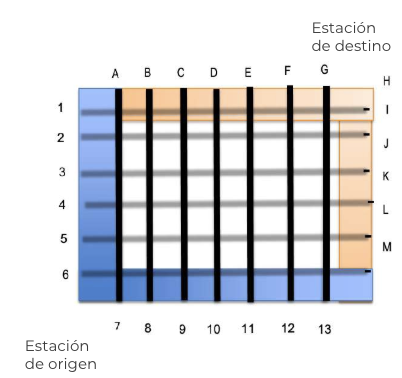
\includegraphics[width=0.50\textwidth]{cuadricula}
	\caption{Cuadrícula ASTI Robotics Challenge}
	\label{fig:5.2}
\end{figure}

El número de estaciones de origen y de destino se conocen de antemano y se numeran con números las estaciones de origen y con letras las estaciones de destino (Figura 5.2).

Para la resolución de esta prueba se requiere de un buen funcionamiento de siguelíneas ya que es la forma en la que el robot va de un punto a otro, siguiendo una línea negra.

Unas peculiaridades de la cuadrícula es que las estaciones de origen y de destino no están conectadas entre sí por tanto no se pueden emplear como puntos intermedios en la ruta calculada sino que solo pueden ser el punto inicial o el final.

Otra peculiaridad es que el usuario puede definir también puntos de la cuadrícula que no están disponibles y que por tanto no se podrán emplear a la hora de calcular el camino más óptimo.

\textbf{Algoritmo A*}

El algoritmo A* es un algoritmo de búsqueda de caminos que busca encontrar la ruta más corta entre dos puntos. 
Combina las estrategias de búsqueda de coste uniforme y búsqueda heurística que permite encontrar soluciones óptimas de forma eficiente.

Este algoritmo es capaz de buscar la ruta más corta desde un nodo inicial (estación de origen) hasta un nodo objetivo (estación de destino).

Para su ejecución se comienza inicializando una lista abierta que contiene los nodos que deben ser evaluados y una lista cerrada que contiene los nodos que ya han sido evaluados.

Cuando el usuario introduce la estación de origen elegida, este punto se añade a la lista abierta como nodo inicial.

Mientras la lista abierta no está vacía, el algoritmo selecciona de forma recurrente el nodo con el menor coste de la lista abierta y lo establece como nodo actual, si este nodo es el nodo objetivo se habrá encontrado una ruta y se puede reconstruir el camino para ejecutarlo después.

Para cada vecino del nodo actual se tiene en cuenta si está o no en la lista cerrada, en caso de estarlo, este nodo se ignorará.
En caso de que no esté en la lista cerrada, se calcula el coste desde el nodo inicial hasta el nodo vecino y si este nodo vecino no está en la lista abierta o el nuevo coste desde el origen es menor que el coste calculado previamente para este vecino se actualizarán los valores de los costes, se establecerá el nodo actual como el padre del vecino y si el vecino no está en la lista abierta, se agregará.

Una vez se encuentra el nodo objetivo, se reconstruye la ruta desde el nodo objetivo hasta el nodo inicial siguiendo los nodos padre.

\subsubsection{5.3.4 Prueba del "laberinto"}\label{laberinto}

En la prueba del laberinto PrimeBot tiene que ir desde la zona de origen hasta el final del laberinto y salir de él (Figura 5.3).
El desarrollo de la prueba tiene que ser totalmente autónomo y evitando tocar las paredes el laberinto.

\begin{figure}[h]
	\centering
	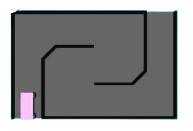
\includegraphics[width=0.50\textwidth]{laberinto}
	\caption{Laberinto ASTI Robotics Challenge}
	\label{fig:5.3}
\end{figure}

Para llevar a cabo esta prueba se utilizan los sensores OPT3101 nombrados anteriormente. 
Esta placa de sensores dispone de 3 canales (TX0,TX1,TX2) con los que podemos detectar objetos a la izquierda del robot, de frente y en el lado derecho proporcionando un ángulo de visión total de 160°.

Para realizar la resolución de los laberintos se ha utilizado la técnica de seguir pared.
El robot seguirá la pared de la derecha o de la izquierda en función de lo que el usuario seleccione vía Bluetooth.

Esta técnica se ha seleccionado ya que la complejidad de los laberintos es baja y no se encuentran laberintos infinitos en los que pueda entrar PrimeBot en bucle.
\newpage
\section{Consideraciones Adicionales}\label{consideraciones}

\textbf{Aspectos que se han tenido en cuenta a la hora de la programación}

\begin{itemize}
\tightlist
\item
  \textbf{Gestión de memoria:} Arduino nano tiene unas capacidades limitadas y con este tipo de algoritmos puede verse limitado en cuanto a memoria a la hora de calcular las rutas, debido a ello se han incorporado funciones que hacen liberación de nodos ya evaluados para reducir el consumo de memoria.
\item
  \textbf{Puntos no disponibles:} se ha tenido en cuenta que los cuatro puntos correspondientes a las esquinas de la cuadrícula no están disponibles y también que cuando el usuario selecciona una estación de origen y una de destino, el resto de estaciones se añaden a la lista de puntos no disponibles para evitar su uso en el cálculo de la ruta.
\end{itemize}


\textbf{Funciones adicionales implementadas en PrimeBot: }
\begin{itemize}
\tightlist
\item
    \textbf{Representación gráfica:} a través del Bluetooth y el monitor Serial, PrimeBot imprime el recorrido que va a realizar para una estación de origen y de destino dadas.
\item
    \textbf{Conectividad Bluetooth:} con la conectividad inalámbrica se pueden indicar las estaciones de origen y de destino, PrimeBot pedirá estos parámetros de forma cíclica para realizar un mayor número de recorridos.
  \item
    \textbf{Caminos alternativos:} además de indicar vía bluetooth las estaciones de origen y destino del recorrido, se pueden indicar puntos de la cuadrícula que estén bloqueados para que a la hora de calcular la ruta se utilicen caminos alternativos.
\end{itemize}

\newpage
\section{Desarrollo web}\label{web}

El objetivo de la web es complementar la información del proyecto PrimeBot y disponer de un lugar donde esté toda la información disponible y las características principales del proyecto de una forma rápida y visual.

Para desarrollar esta web se ha utilizado un dominio personal en el que no se ha utilizado ningún gestor de contenidos.

Toda la programación se ha realizado con HTML5 + CSS + JavaScript.

Además se añaden documentos gráficos como vídeos de la realización de diferentes pruebas.
\begin{figure}[h]
	\centering
	\includegraphics[width=1\textwidth]{CapturaWeb}
	\caption{Web del proyecto}
	\label{fig:5.5}
\end{figure}
\capitulo{6}{Trabajos relacionados}

En el ámbito de la robótica, la realización de Robots siguelíneas es muy habitual y hay un gran número de ejemplos en la comunidad.
También hay muchos ejemplos de robots que resuelven laberintos de forma autónoma.


\section{Proyectos}\label{proyectos}

\subsection{Robot Siguelíneas - Pumatron}\label{siguelineas}

El mayor exponente de robots siguelíneas que podemos encontrar en la comunidad española permanece al equipo de la Liga Nacional de Robótica de Competición llamado 'Puma Pride'

El robot Pumatron desarrollado por este equipo ha ganado una gran cantidad de carreras siguelíneas obteniendo un rendimiento y una velocidad extraordinarias.

\subsection{Micromouse}\label{micromouse}

Los robots de competición Micromouse son una de las inspiraciones del proyecto PrimeBot siendo unos robots de formato compacto que son capaces de resolver laberintos muy complejos.~\cite{koza92}


Su formato extremadamente compacto junto a su gran potencia y velocidad hacen que sus competiciones sean realmente emocionantes.
\capitulo{7}{Conclusiones y Líneas de trabajo futuras}

En esta sección se exponen las conclusiones derivadas del trabajo, así como las posibles evoluciones futuras de PrimeBot para realizar nuevas versiones del proyecto.

\section{Conclusiones}\label{conclusiones}

Tras el desarrollo del proyecto podemos concluir que:

\begin{itemize}
\tightlist
\item
 El objetivo principal del proyecto se ha cumplido correctamente, llegando a la solución para cada una de las pruebas seleccionadas inicialmente e incluso añadiendo funcionalidades no contempladas en un inicio.
\item
 El uso de una forma de desarrollo ágil como SCRUM y el sistema de Sprints ha permitido realizar un desarrollo ordenado y eficaz aprovechando al máximo los recursos.
\item
 Gracias a la parte de investigación y búsqueda de elementos, proyectos y trabajo realizado con la comunidad Open Source, se ha podido llegar a una solución muy buena para cada una de las pruebas.
\item
 El empleo del ecosistema Arduino y la gran comunidad, además de la cantidad de sensores y elementos compatibles directamente con la plataforma han permitido poder contemplar muchas opciones para cada una de las soluciones que iba a realizar PrimeBot.
\end{itemize}

\section{Trabajo futuro}\label{trabajo-futuro}

A lo largo del desarrollo del proyecto han salido nuevas versiones de Arduino que sería interesante implementar en las versiones posteriores de PrimeBot.

\begin{itemize}
\tightlist
\item
 Incorporación de STM32: las nuevas versiones de arduino han incorporado el microcontrolador STM32 que puede incorporar una gran mejora de rendimiento para este tipo de proyectos, siendo ese microcontrolador uno de los más populares en proyectos de robots siguelíneas.
\item
 Preparación del resto de pruebas: actualmente PrimeBot en su primera versión no realiza todas las pruebas disponibles en el ASTI Robotics Challenge, una nueva línea de implementación sería realizar el código para afrontar el resto de pruebas disponibles.
\end{itemize}



\bibliographystyle{plain}
\bibliography{bibliografia}

\end{document}
